% LaTeX layout by Jonas Kahler, jonas@derkahler.de
% AutoTux Final Report
% Group Tux:
% Max Enelund, Jerker Ersare, Thorsteinn D. Jörundsson,
% Jonas Kahler, Dennis Karlberg Niklas le Comte, Marco Trifance, Ivo Vryashkov
% Chapter 1 - Project Organization and Milestone Planning
\chapter{Algorithmic Fundamentals}
%% Environment Detection
\section{Environment Detection}
%%% Image Processing by Max
\subsection[Image Processing]{Image Processing\textsuperscript{[ME]}}
The first step towards a desired steering angle is processing the image. The
ideal result of the image processing would be an image with perfectly applied
edge detection, where all the edges are one colour and the rest is another. We
decided to turn all edges white and everything else black.\\
We started out by using OpenCV to convert our colorspace image into grayscale.
By using the \textit{threshold} function from OpenCV it was easy to filter out a
certain spectrum of brightness in the image and drawing contours around the
remaining edges was done with a mixture of \textit{findContours} and
\textit{drawContours}.\\
This resulted in an image that was only black with white contours around
objects, but due to how the \textit{threshold} function was built it was rather
hard to achieve a consistent good quality image because of the different
lightning conditions in the room. To counter this problem we tried to create an
adaptive threshold using the light sensor on the front facing ultrasonic sensor,
this did increase the quality of the image. But while testing this we stumbled
upon OpenCV's \textit{Canny} function.\\

\noindent
\textit{Canny} is a function specifically made for edge detection, it uses the
\textit{Canny86} algorithm (See Algorithmic References for more information
about \textit{Canny}).\\
Using this we get an acceptable image to work with at almost all times. We
noticed that the algorithm itself might be a bit resource heavy but not so heavy
that it would pose as a problem, especially not when we only analyze half the
image as explained in section ~\ref{impdetailslbl}:
\hyperlink{impdetailstgt}{Implementation Details}.

%%% Lane Detection by Dennis
\subsection[Lane Detection]{Lane Detection\textsuperscript{[DK]}}
When the image is processed with clear edges it is time to apply lane detection
logic. Every iteration we loop through pixels horizontally and vertically,
looking for white or light-grey pixels. For the left and right lane markings,
the pixel we start looking from is vertically a pixel very close to the bottom
of the picture, we refer to it as our control scanline. Horizontally, we start
from the middle of the picture. We then loop through the pixels to the left and
right of the starting point, looking for white pixels. The number of pixels
looped through before finding the desired pixel is then stored and used as a
distance measurement when applying the lane following.\\

\noindent
The stop-line detection works the same way as the detection of the left and
right lane markings. When looking for stop-lines however, we have two separate
starting points, they are offset +/- 50 pixels to the left and right of the
starting point we used in the lane marking detection. We then loop through
pixels on the vertically instead of horizontally. The reason we check the
stopline at two separate locations is to simply increase robustness, more
specifically in this case these two distances are compared to check whether the
line detected is more or less horizontal. Additional robustness in this
detection is achieved by checking this for a few iterations before actually
treating it as a stop-line. If these robustness checks are passed, we forward
the distance to the stop-line to the DecisionMaker, in which we adjust the speed
appropriately. Before this is done however, we ran a few tests and concluded
that there was no point in sending any stop-line distances if the line was to
far away. Infact, we ended up only sending the distance if it was low enough
that the DecisionMaker would consider stopping. This was not the initial idea,
at first we wanted to send farther distances and have a certain distance at
which the car slows down up until it reaches the threshold of stopping. However,
seeing as we had some issues getting the car to run at higher speeds with our
current implementation, we felt that there was no purpose in slowing down due to
the car's speed already being low enough to simply stop. The car also stopped
very smoothly when setting the speed to 0.\\

\noindent
Furthermore, when no lane markings are found on either side during the
lane-detection, a flag we call “quality” is set to false. What this means is
that the data from the LaneFollower is not to be trusted when it comes to
decision making. The intention was that this value were to be handled in the
DecisionMaker, potentially lowering the speed and perhaps even setting the
steering wheel angle to 0. We unfortunately did not have time to handle this in
the DecisionMaker although it was handled in the Lane Follower.
\begin{figure}[ht]
  \centering
  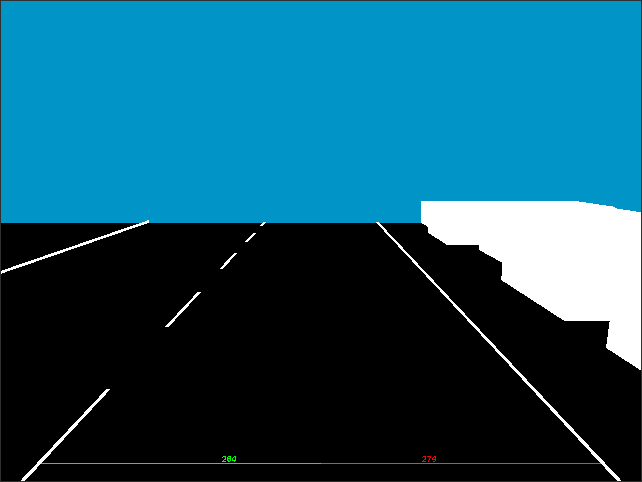
\includegraphics[width=1\textwidth]{X-LaneFollowerScr.png}
  \caption{LaneFollower in the simulation}
  \label{lfsim}
\end{figure}


%%% Ultrasonic Sensors by Jerker
\newpage
\subsection[Ultrasonic Sensors]{Ultrasonic Sensors\textsuperscript{[JE]}}
The ultrasonic sensors use the I²C protocol for communication. As discussed
further in section ~\ref{hwintlbl}: \hyperlink{hwinttgt}{Hardware-Software
Integration}, this link seems sensitive to fluctuations in voltage,
and although we reduced this sensitivity by mounting external pull-up resistors
connected to the I\textsuperscript{2}C bus, the sensors can still respond with
unexpected 0's occasionally instead of the current distance measured. Therefore,
we discard any readings of 0 until it occurs at least three consecutive times.\\

\noindent
All values are averaged with a circular buffer, currently having the size of 4
elements. These mechanisms may reduce reaction time slightly for sudden
obstacles, but we considered the reduction in noise to be worth this, taking
into account which challenges the miniature car was expected to handle.\\

\noindent
Values are capped to 90 cm (anything above this will still be sent as 90),
because values above this will likely be unusable, noisy fluctuations not
directly interesting to the current state of the car.\\

\noindent
The light sensor of the front ultrasonic sensor is also read, and used to
determine the strength of the headlights. Earlier we discussed the possibility
of adjusting the camera image processing threshold values based on the light
sensor reading, which is why the light sensor reading is also transmitted to the
high-level board.

%%% Infrared Sensors by Jeker
\subsection[Infrared Sensors]{Infrared Sensors\textsuperscript{[JE]}}
The infrared sensors are read using the analog-to-digital converters of the
STM32. We based our formula for translating sensor voltage levels to distance on
a formula designed for Arduinos, which have a lower ADC resolution. To
compensate for the difference in resolution, we simply bitshift the values.\\

\noindent
To minimize noise, each time we read the sensor values we let the ADC read 4
samples for each sensor. Then we translate the average sampled voltage level for
each sensor into a distance value, which is in turn averaged with the previous
distance value.\\

\noindent
Values are capped to 28 cm, because any values above this will be unusable,
noisy fluctuations.

%%% Wheel Encoder by Thorsteinn
\subsection[Wheel Encoder]{Wheel Encoder\textsuperscript{[TDJ]}}
The wheel encoder works by measuring wheel revolutions using infrared
reflections. In a proper setup, it should be possible to not only measure
distance traveled, but speed as well. However, fitting the wheel encoder
properly was hard and the results were at times unpredictable.\\

\noindent
The circumference of the wheel measured was 20.42 cm. This wheel had nine
stripes on its interiors, which reflected the infrared light back to the sensor.
After a meter of travel, the sensor should have measured ~44 stripes. These
measurements could be used to calculate both speed and distance traveled using
the amount of stripes per meter.\\

\noindent
Initially, the wheel encoder ran within its own thread. The rate of reliable
results was not satisfactory with this setup, so it was setup to rely on
interrupt routines which were triggered when a new value was read. This
increased the reliability of results quite significantly, but was still
insufficient at operating speeds with an inaccuracy of 10 - 15\%\\

\noindent
The particular wheel encoder used is clearly specified by the manufacturer as
only intended for a specific wheel (different from the wheels used in this
project). If we would have had more time, we would consider using for example a
computer mouse to measure distance travelled.

%% Vehicle Control by Jerker
\section[Vehicle Control]{Vehicle Control\textsuperscript{[JE]}}

%%% Safety Mechanism
\subsection{Safety Mechanism}
If no valid control data is received through the serial connection for a given
time, the wheels are centered and the engine is stopped. This constitutes a
basic safety mechanism for a broken connection or execution problems on the
high-level board.

%%% Steering Control
\section{Steering Control}
The steering wheel angle is forwarded agnostically from the high-level board to
the servo. In the OpenDaVinci components, radians are used. In the proxy, these
are converted to degrees, centered around 90 degrees to make sure we can use
unsigned bytes for transmitting. Hence 90 degrees means forward, 60 means full
left turn and so on. We roughly see 30 degrees or about 0.5 radians as the
maximum turning angle in each direction.

%%% Engine Control
\subsection{Engine Control}
For controlling the engine power, we use a set of prefixed pulsewidth values.
The high-level board sends an integer number, where 0 means reverse, 1 means
neutral, 2 means forward slowly, and 3 means cruise speed forward. Speeds above
1.0  in the OpenDaVINCI-based components are seen as cruise speed. The
conversion occurs in the proxy component. The solution of indexed speed modes
has safety benefits, and indeed we did not have the problems of unexpected
engine power surges that several other groups did.\\

\noindent
We do not use any speed regulator mechanism to adjust the engine power based on
how the current speed relates to the desired speed, and therefore had to
manually adjust the PWM values to use the car with low battery power. We deemed
the speed measurement from the wheel encoder to be too unreliable to use as a
basis for adjusting the engine power. If we would have had the time to explore
more reliable ways to measure speed or distance, a speed regulator could have
been helpful.

%%% Light Control
\subsection{Light Control}
Using the neopixel LED strips, we gave the car headlights, tail lights, brake
lights, indicator lights, reverse light and an RC mode light (blue). The reverse
light, indicator lights (flashing orange) and brake lights are controlled by the
components running on the high-level board. The RC mode light is automatic. The
tail lights are always lit, and the headlights have a strength that adapts to
the surrounding light levels (as measured by the light sensor in the front
ultrasonic sensor),  which can help reduce the camera’s exposure time in dark
environments.